\chapter{系统架构}

本文提出一个基于可编程网卡的高性能数据中心系统架构。
可编程网卡是服务器与外界通信的 ``网关'',也是服务器内硬件设备、虚拟机间通信的 ``枢纽''。
我们把虚拟化、网络和存储功能、操作系统中需要高性能的数据平面卸载到可编程网卡,以降低 ``数据中心税'',让 CPU 集中精力于客户的应用程序。


\begin{figure}[htbp]
	\centering
	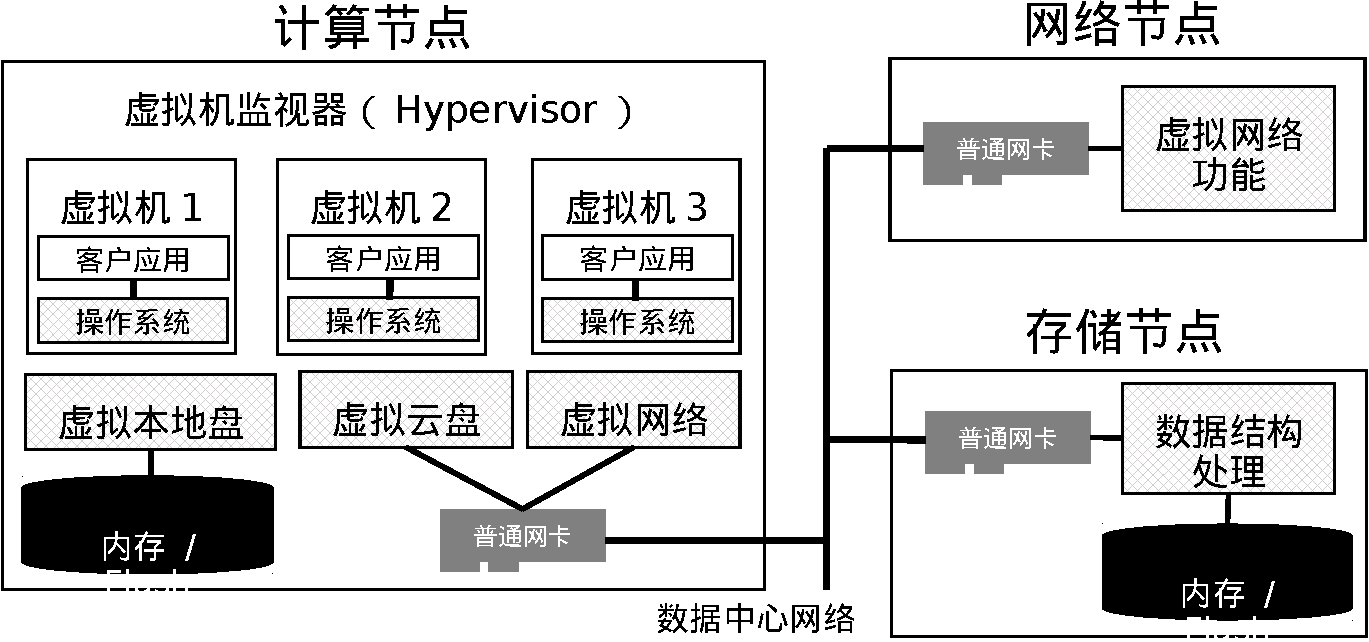
\includegraphics[width=0.8\textwidth]{figures/virt_arch.pdf}
	\caption{回顾:虚拟化的数据中心架构。}
	\label{arch:fig:virt-architecture}
\end{figure}

第 \ref{chapter:intro} 章已经讨论过,如图 \ref{arch:fig:virt-architecture} 所示,虚拟化的数据中心主要可以分为计算、网络、存储节点。
在网络和存储节点,我们采用控制面与数据面分离的设计思想。数据面是操作相对频繁、逻辑相对简单的处理,而控制面是操作相对不频繁、逻辑相对复杂的处理。我们在可编程网卡中实现数据面,在主机 CPU 上实现控制面。这包括第 \ref{chapter:clicknp} 章的虚拟网络功能和第 \ref{chapter:kvdirect} 章的数据结构处理。加速虚拟网络功能和远程数据结构访问也是本文最重要的创新。

在计算节点,亦即客户虚拟机所在的服务器主机上,我们用可编程网卡实现虚拟机监控器(hypervior)的虚拟化功能和高层抽象。
虚拟化分为 ``一虚多'' 和 ``多虚一'' 两个方面。
``一虚多'',即可编程网卡把计算节点内的硬件资源虚拟化成多个逻辑资源,实现外部机器和本地虚拟机的多路复用。例如,第 \ref{chapter:clicknp} 章的 ClickNP 将硬件网卡和网络链路虚拟化为多个租户的虚拟网络;第 \ref{chapter:socksdirect} 章的 SocksDirect 实现了容器网络。
``多虚一'',即可编程网卡把数据中心内物理上分散的资源虚拟化成一个逻辑资源,实现逻辑资源到物理资源的映射和路由。例如,第 \ref{chapter:clicknp} 章的 ClickNP 将数据中心内网络功能虚拟化成逻辑上统一的网络功能;第 \ref{chapter:clicknp} 章的 KV-Direct 客户端将分布式键值存储虚拟化成一个大的哈希表;还可以实现存储和内存的解聚(disaggregation)。
高层抽象分为操作系统原语和数据结构操作原语两个方面。
为了加速操作系统原语并控制硬件的复杂度,我们把操作系统原语分为可编程网卡上的可靠通信协议和主机 CPU 上运行的用户态库、用户态管理程序,如第 \ref{chapter:socksdirect} 章的套接字通信原语。
为了提供数据结构操作原语,应用程序通过轻量级用户态库直接访问网卡,如第 \ref{chapter:kvdirect} 章的键值操作原语。

图 \ref{arch:fig:accel-arch} 显示了基于可编程网卡的系统总体架构。下面我们将按照网络、存储和高层抽象的顺序,简要介绍本文后续各章的总体设计。


\begin{figure}[htbp]
	\centering
	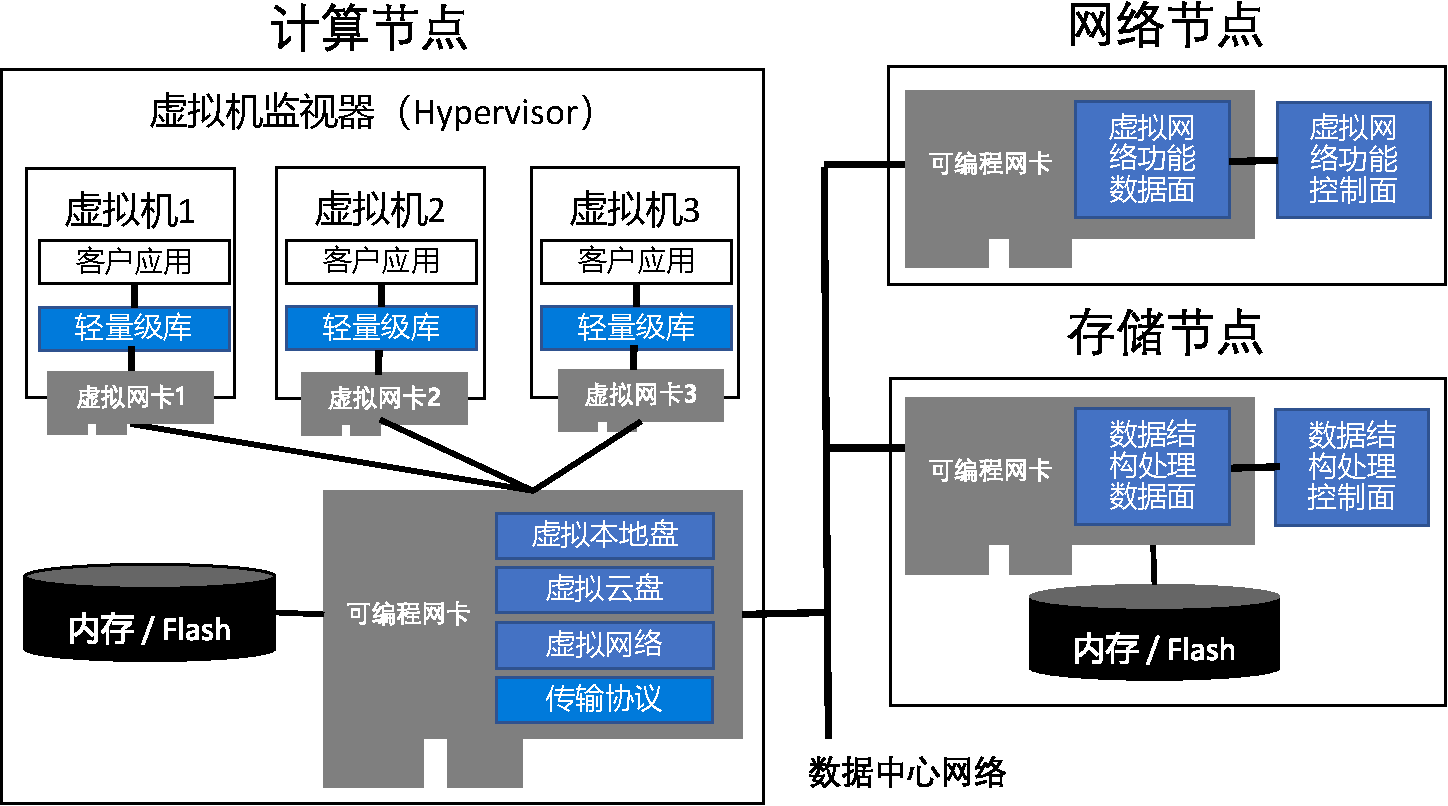
\includegraphics[width=0.8\textwidth]{figures/accel_arch.pdf}
	\caption{基于可编程网卡的数据中心系统总体架构。}
	\label{arch:fig:accel-arch}
\end{figure}



\section{网络加速}

\subsection{网络虚拟化加速}

\begin{figure}[htbp]
	\centering
	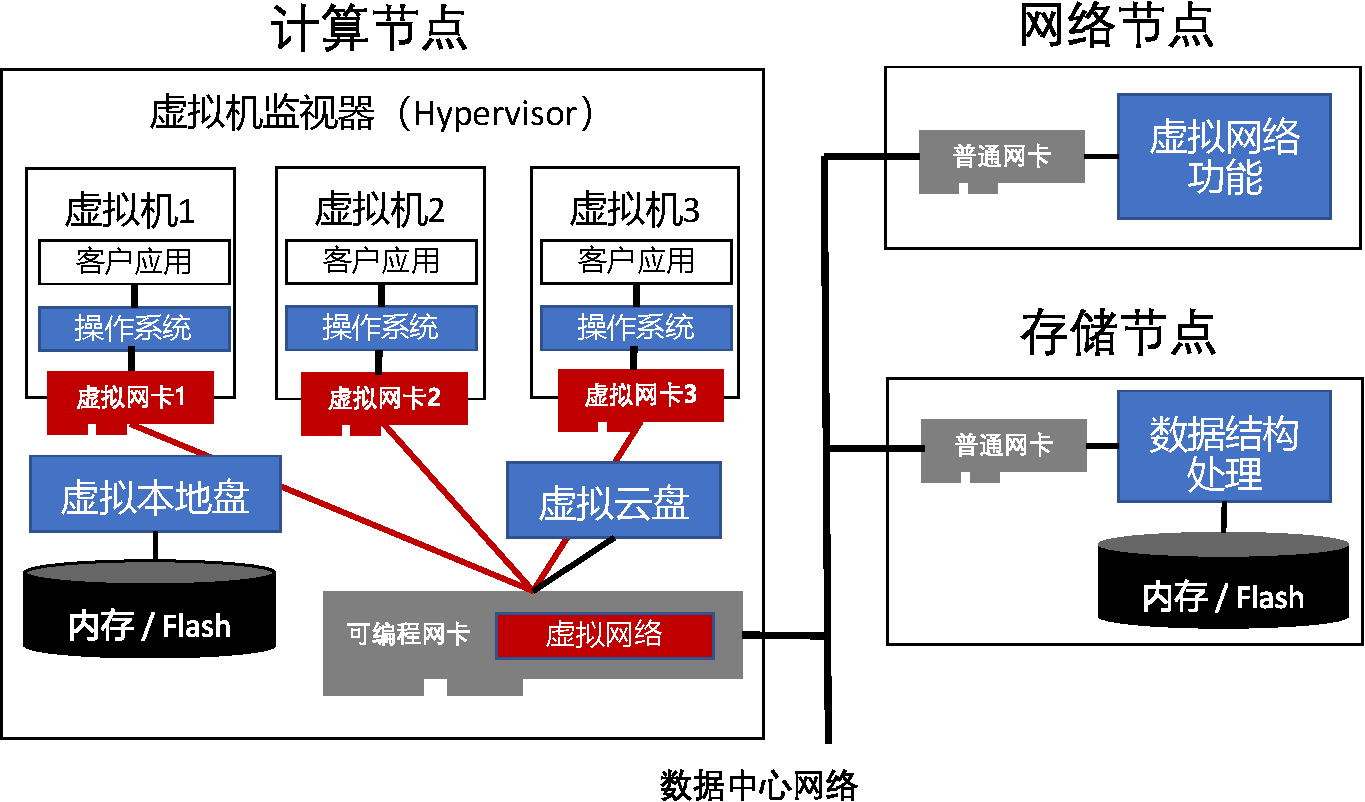
\includegraphics[width=0.8\textwidth]{figures/virtual_network.pdf}
	\caption{用可编程网卡加速虚拟网络后的架构。}
	\label{arch:fig:virtual-network}
\end{figure}

\subsection{网络功能加速}


位置:存储、网关等节点。CPU bypass(控制面数据面分离,数据面 offload,控制面仍在 CPU 上)


直接处理网络数据包并直接返回,数据面无需经过 CPU(ClickNP NF offload)。


\begin{figure}[htbp]
	\centering
	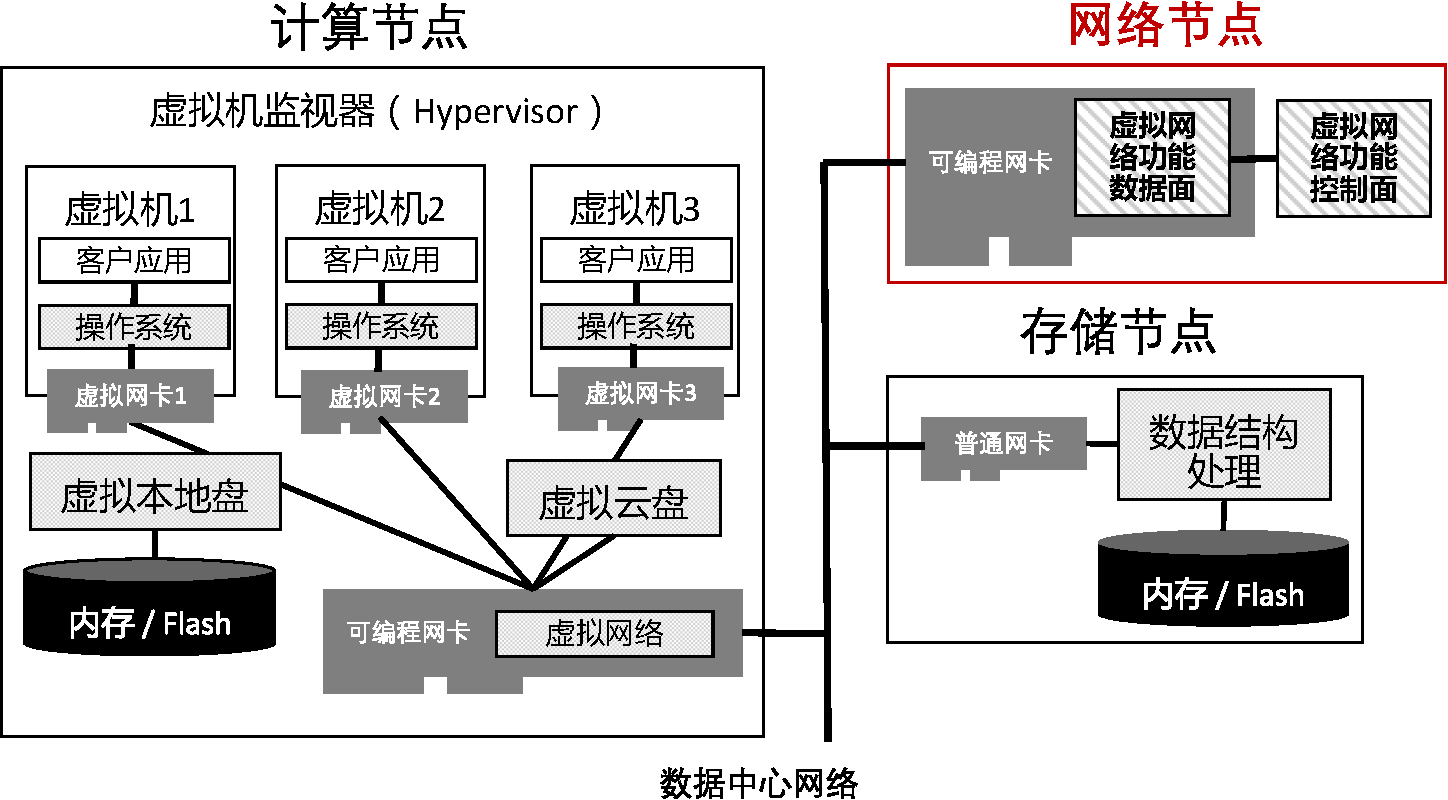
\includegraphics[width=0.8\textwidth]{figures/NFV_accel.pdf}
	\caption{用可编程网卡加速网络功能后的架构。}
	\label{arch:fig:network-function}
\end{figure}

\section{存储加速}

\subsection{存储虚拟化加速}

\begin{figure}[htbp]
	\centering
	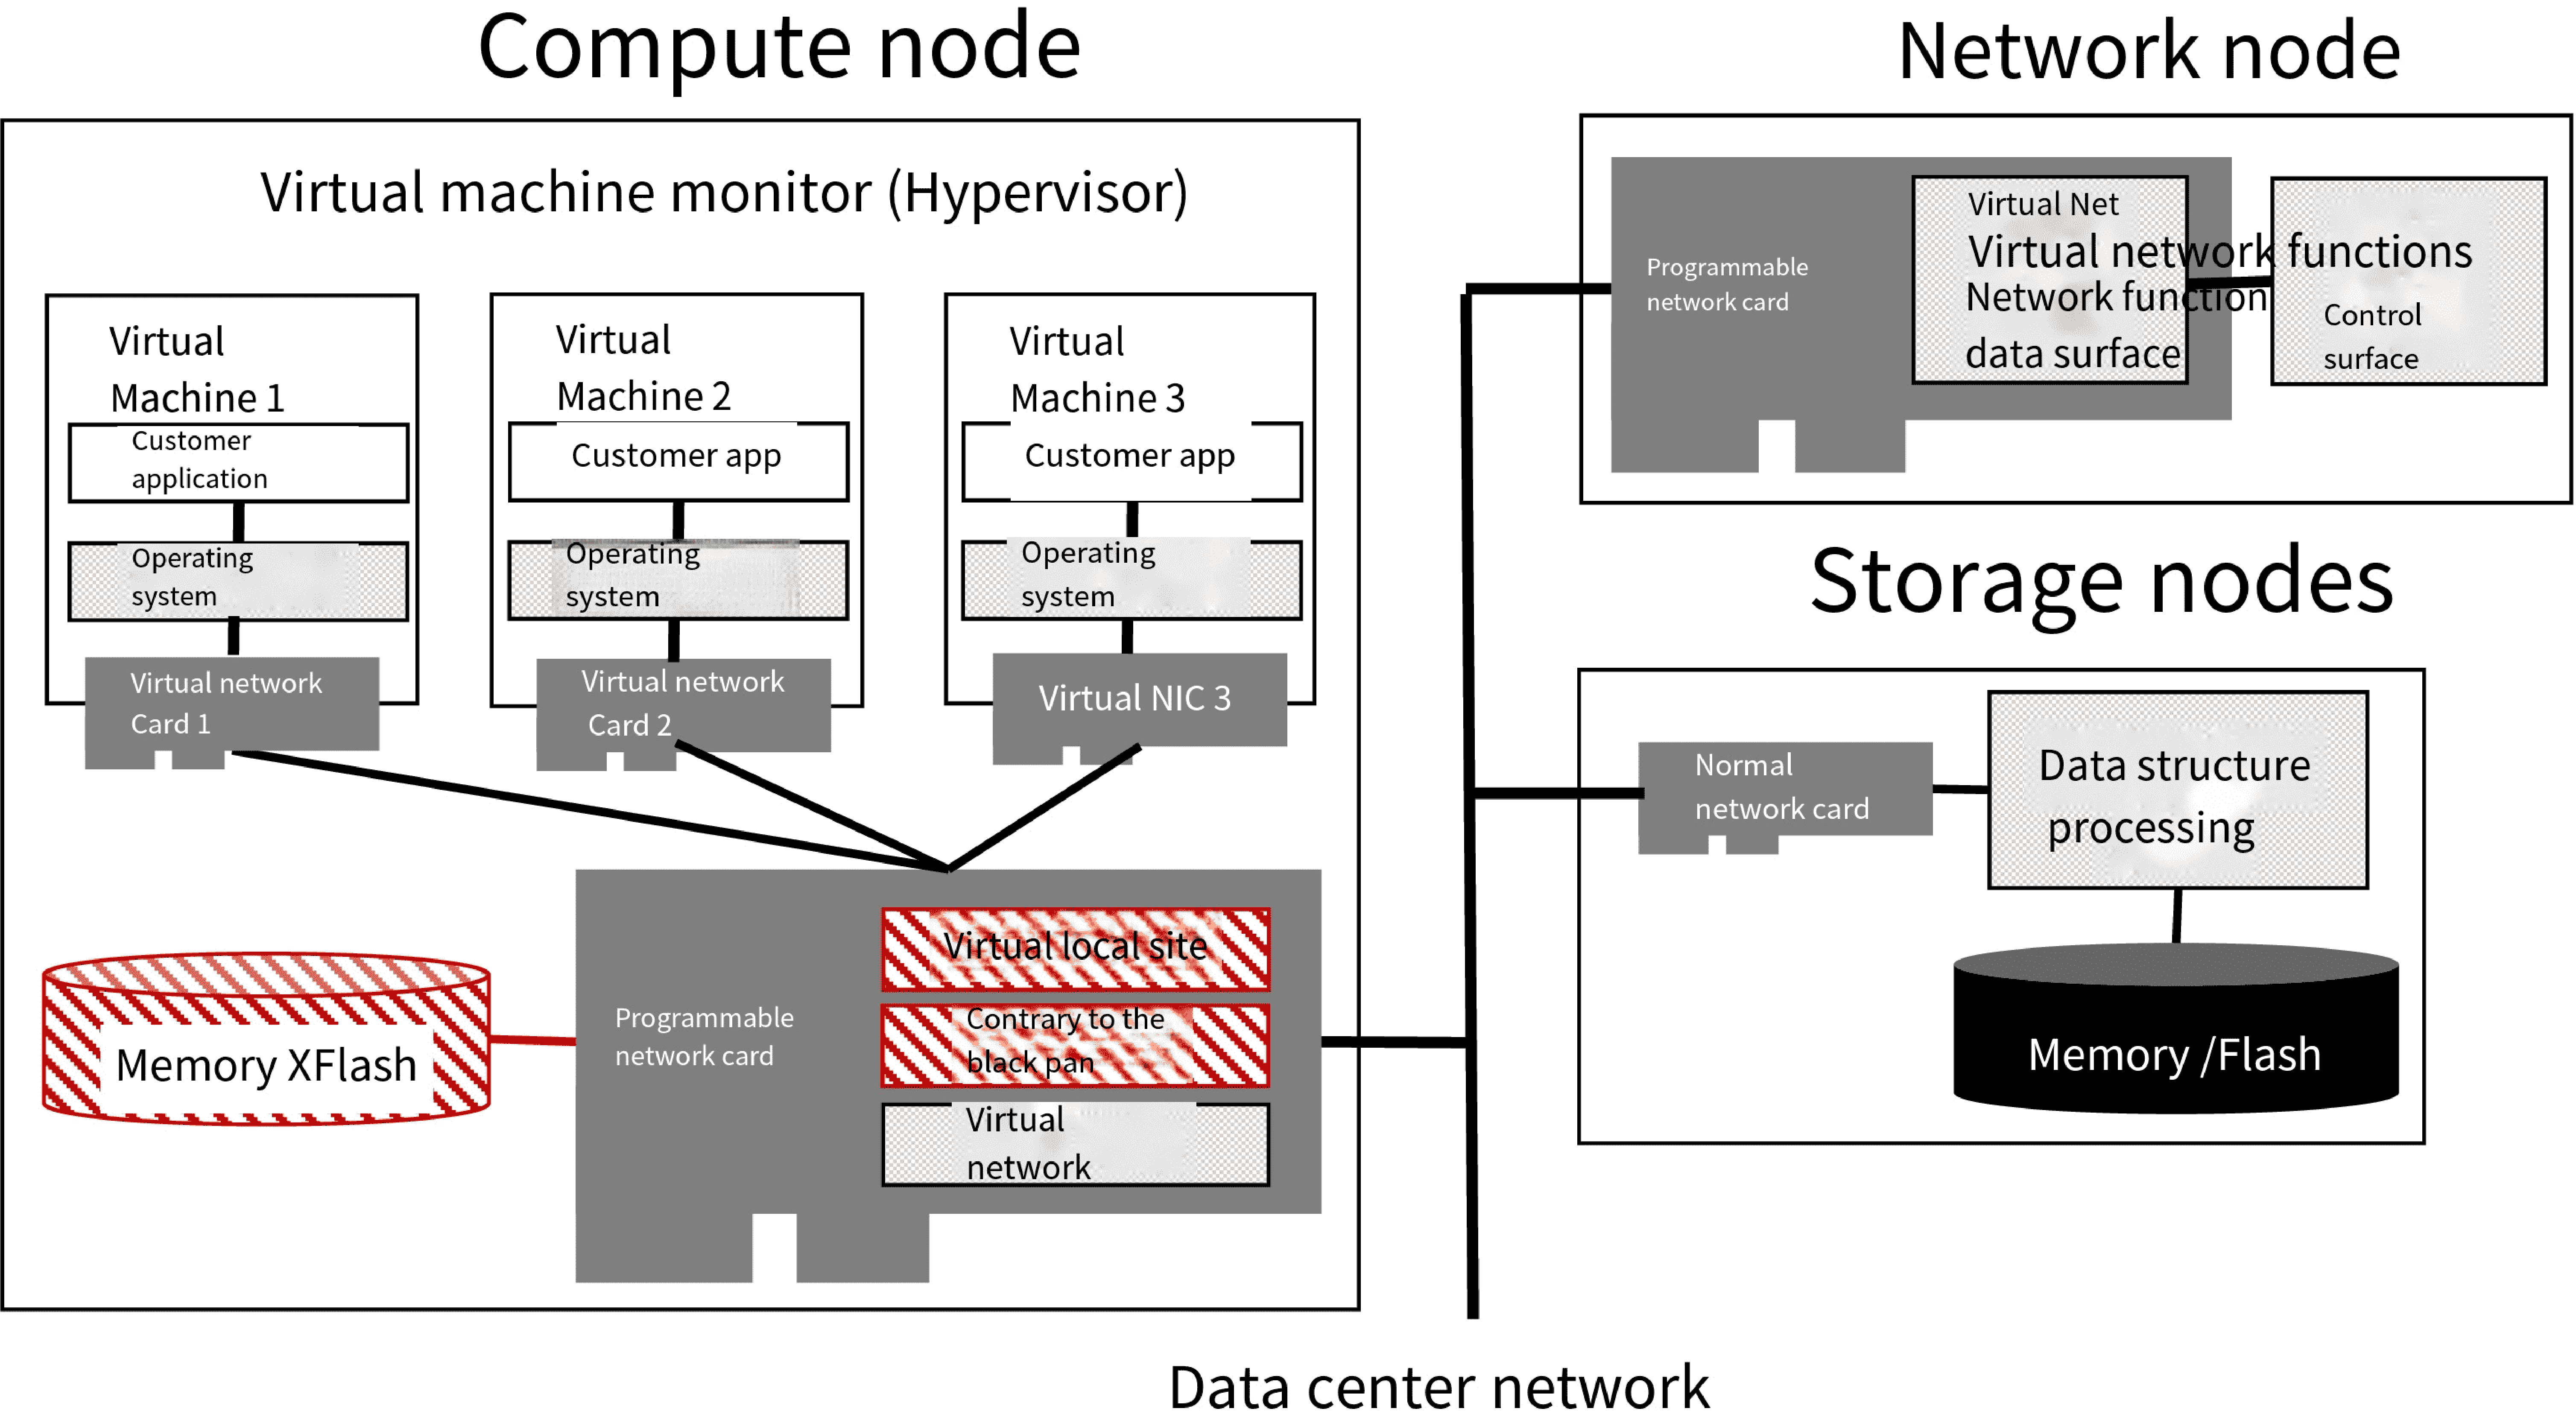
\includegraphics[width=0.8\textwidth]{figures/virt_storage.pdf}
	\caption{用可编程网卡加速本地存储和云存储后的架构。}
	\label{arch:fig:virt-storage}
\end{figure}

\subsection{数据结构处理加速}


网卡直接访问内存数据结构

直接访问远程硬件资源,而无需经过远程机器的 CPU (KV-Direct内存数据结构的服务器端,还可以访问闪存(SSD)记录日志后直接返回 ACK,缩短处理延迟)。

\begin{figure}[htbp]
	\centering
	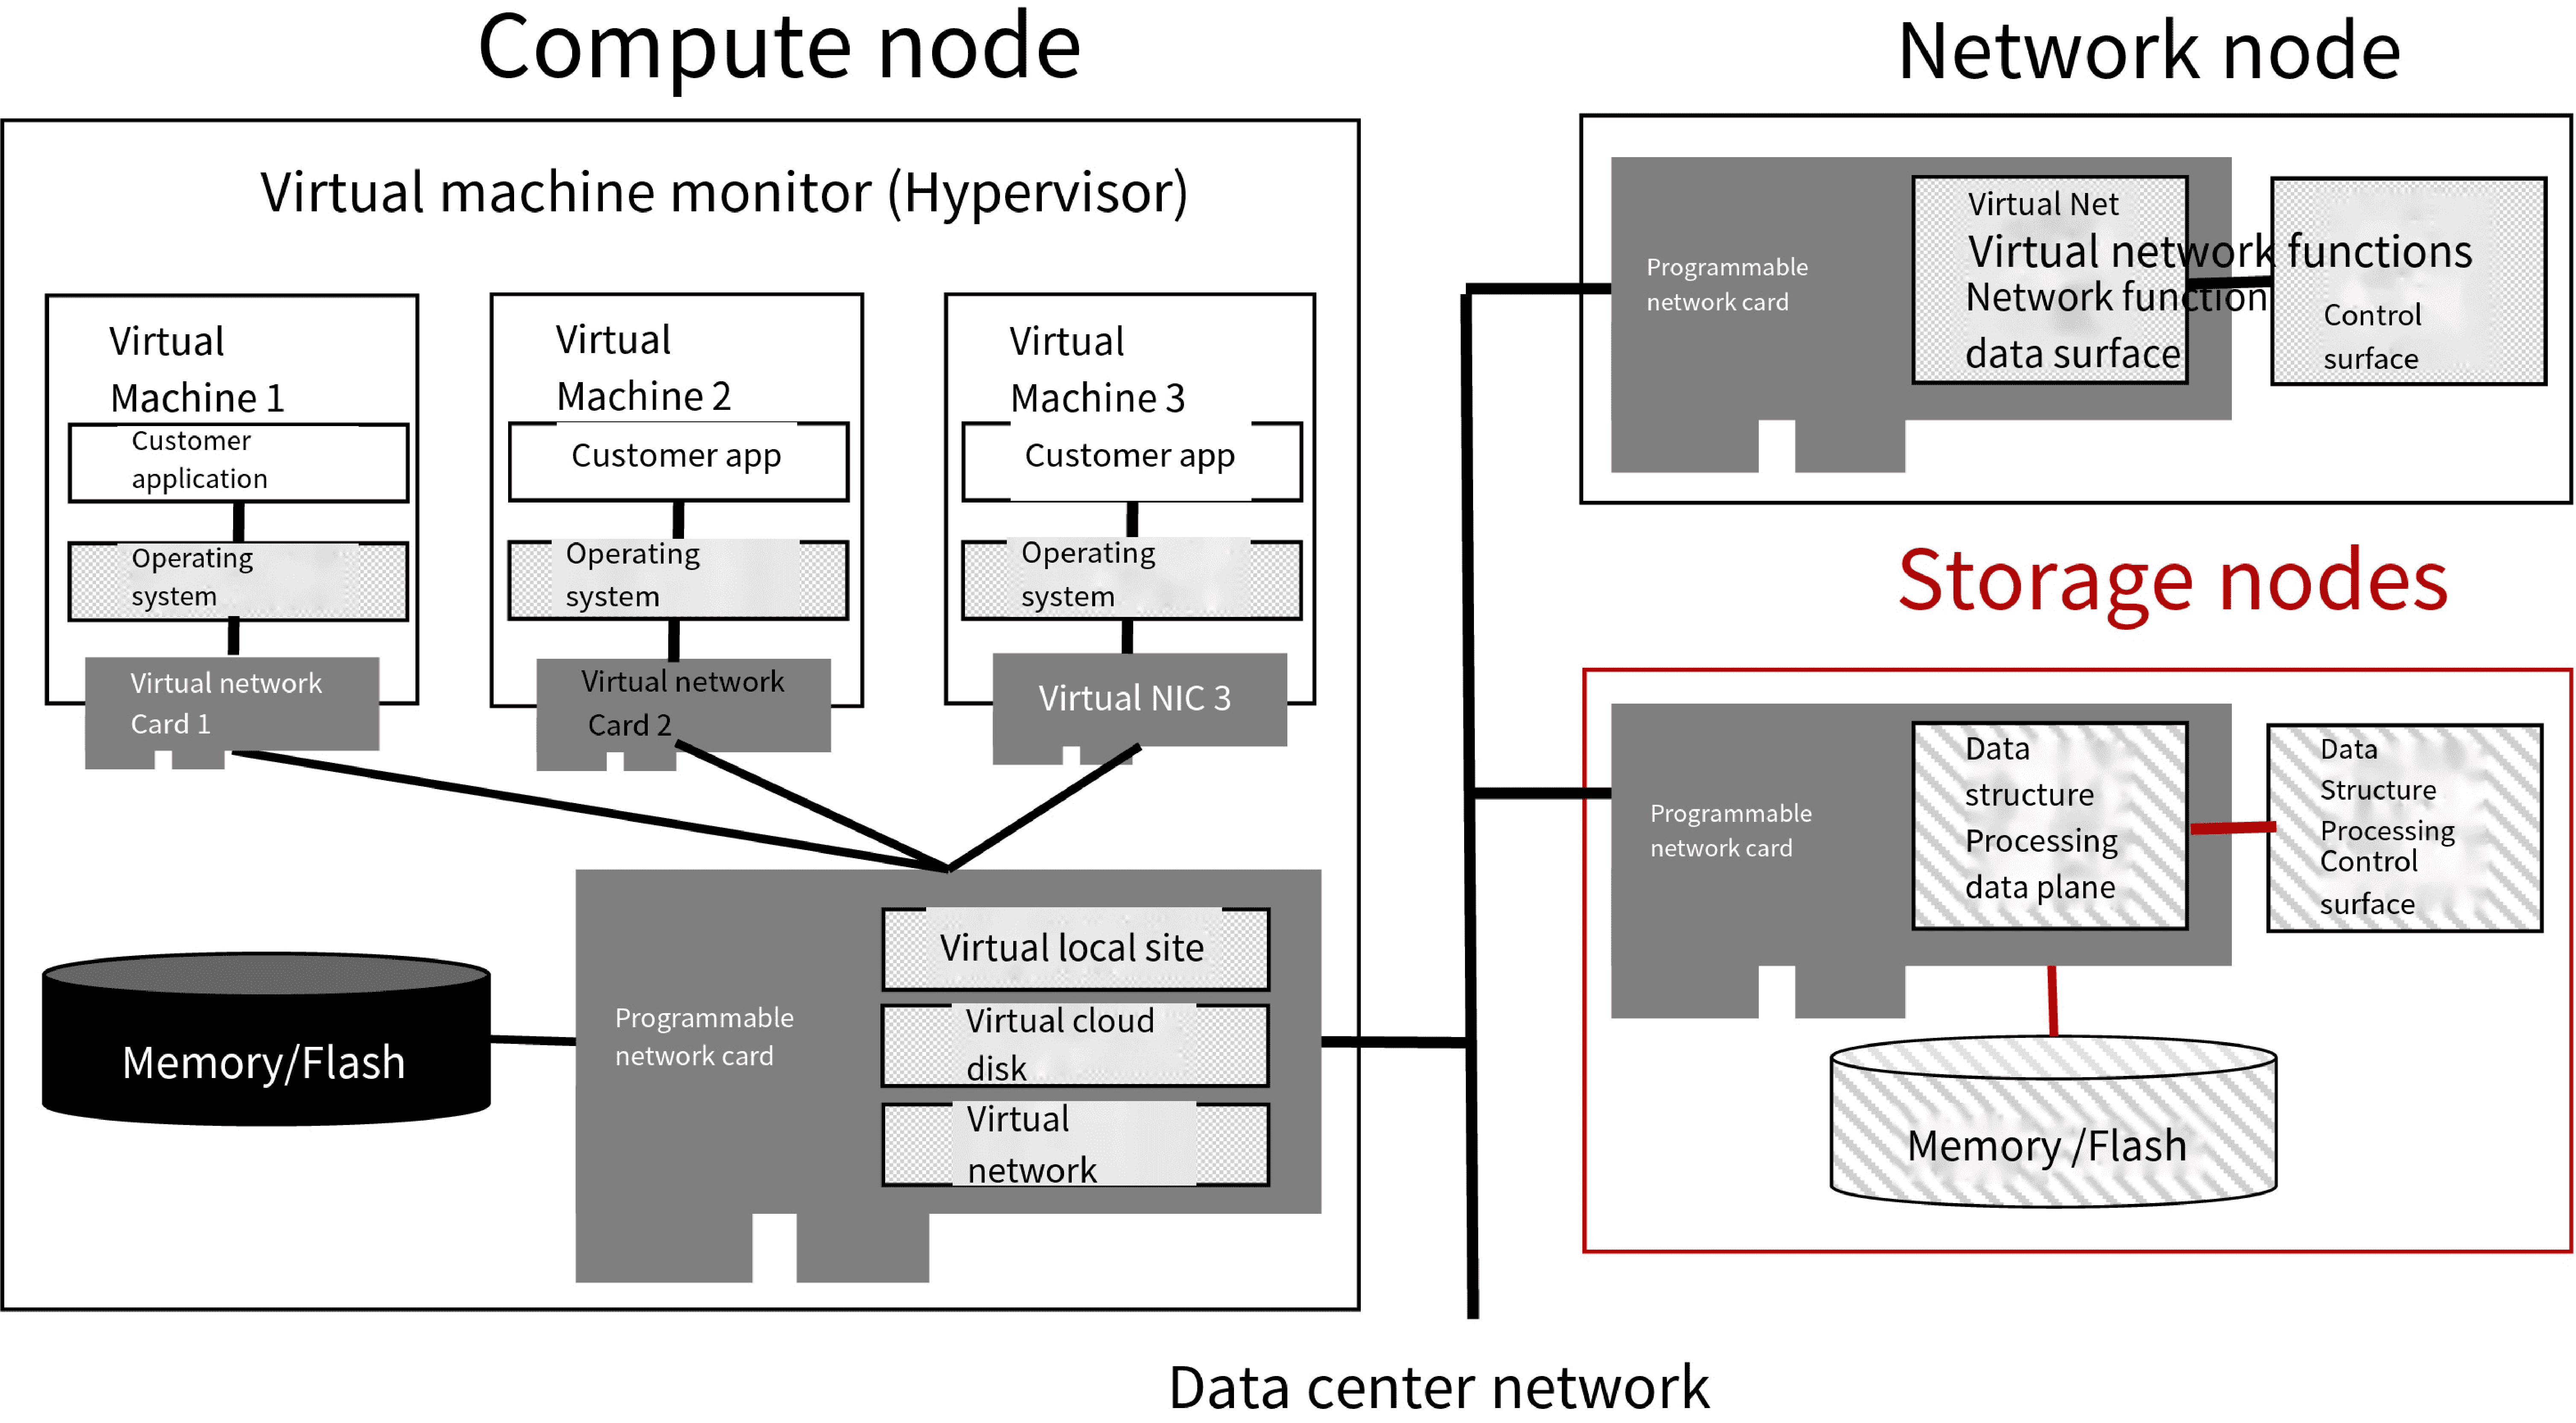
\includegraphics[width=0.8\textwidth]{figures/data_structure_accel.pdf}
	\caption{用可编程网卡加速数据结构处理后的架构。}
	\label{arch:fig:data-structure-accel}
\end{figure}

\section{操作系统加速}

OS kernel 给应用程序提供的原语可以重构为(控制面)协调和管理(仍在内核或用户态 daemon) + (数据面)用户态 library 负责高层抽象 + (数据面)可编程网卡负责多路复用、调度唤醒和可靠传输等低层语义,需要思考数据面上软硬件的接口(SocksDirect)。

\begin{figure}[htbp]
	\centering
	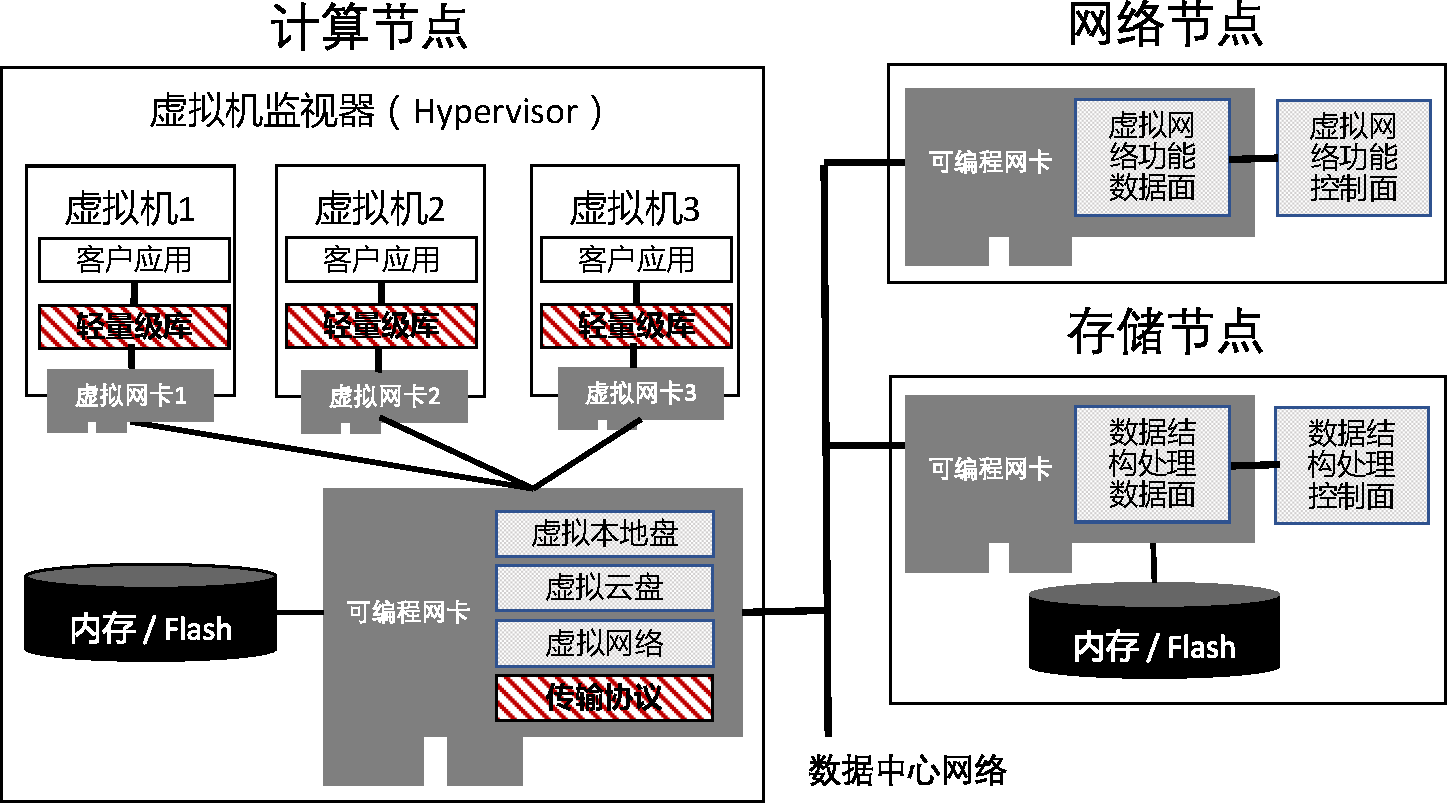
\includegraphics[width=0.8\textwidth]{figures/os_primitives_accel.pdf}
	\caption{用可编程网卡加速操作系统通信原语后的架构。}
	\label{arch:fig:os-primitives-accel}
\end{figure}


\section{可编程网卡}



\begin{figure}[htbp]
	\centering
	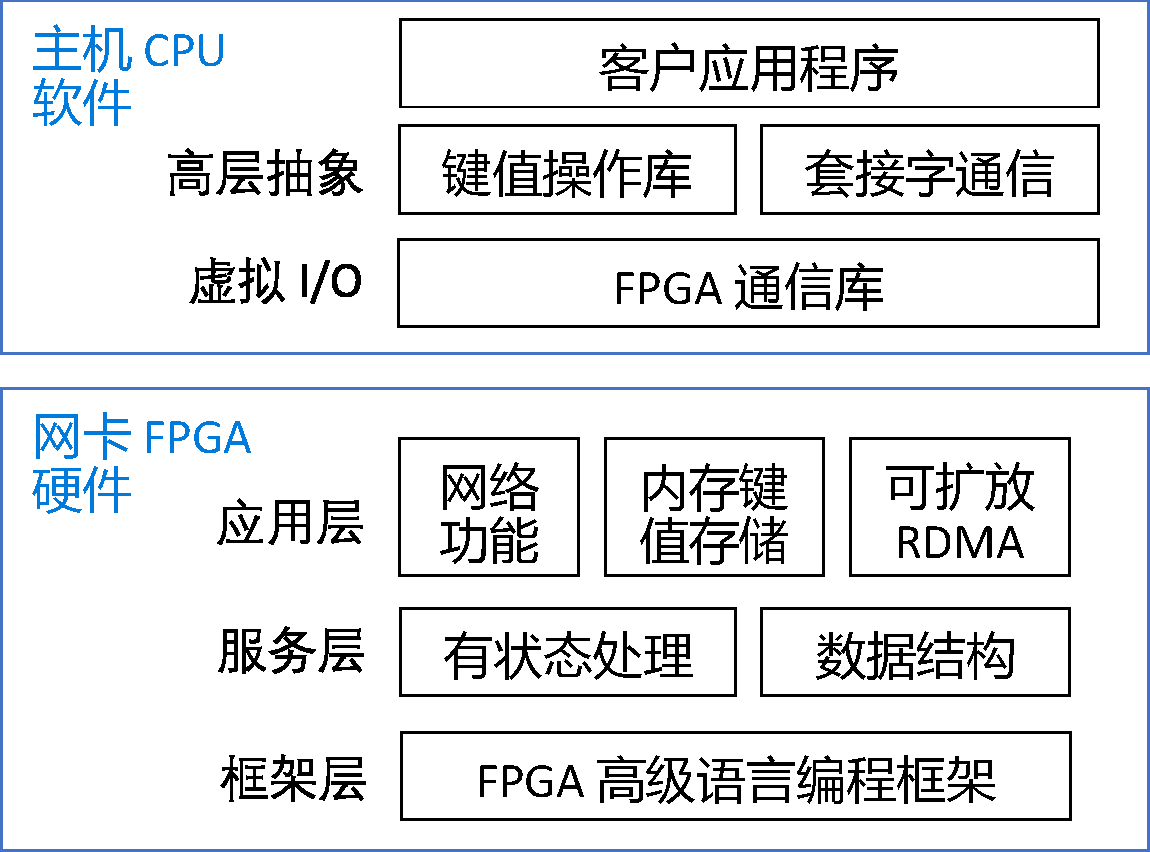
\includegraphics[width=0.6\textwidth]{figures/sw_hw_codesign.pdf}
	\caption{软硬件协同设计的可编程网卡架构。}
	\label{arch:fig:sw-hw-codesign}
\end{figure}


\subsection{硬件架构}

可编程网卡需要高度灵活性。为什么要 FPGA + CPU + ASIC SoC。回应第二章。

\textbf{图1: 网卡 SoC 结构图}

\subsection{高级语言编程框架}

FPGA 高级语言编程:ClickNP,适合流式处理的模块化 FPGA 高级语言编程

\subsection{基础服务中间件}

有状态处理(stateful processing)、数据结构、可扩放 RDMA

本文使用高级语言编程框架实现基础服务中间件,中间件未来可以硬件化。

\subsection{主机上的用户态运行库}

